\chapter{Results and Discussion}
\index{Results and Discussion@\emph{Results and Discussion}}%
\label{chap:results}

\section{Evaluation}\label{sec:results-evaluation}

We begin our discussion by first stepping back and performing a meta-validation 
of the ErLam toolkit itself, before comparing the scheduling mechanisms amongst 
themselves. We ask:
\vspace{-3mm}\begin{itemize}
    \item How complex must our implementations be to create our test primitives? 
    \item For each scheduler, does our implementation work as expected, despite a minimalistic scheduler API?
    \item Does the channel implementation lend itself to scheduling decisions? If so, in what cases?
\end{itemize}\vspace{-3mm}
These questions will evaluate ErLam, both as a language and runtime, but also as a 
simulator for scheduler experimentation, comparison, and evaluation. We attend to
these questions in order;
Section~\ref{sec:results-test-case-implementation} critiques the language as a 
medium for simulation design through the development of our test primitives.
Section~\ref{sec:results-evaluation-classical} discusses our evaluation of the
scheduler API using several of the testing primitives on the aforementioned 
classical schedulers. 
Then in section~\ref{sec:results-channel-implementations}, we discuss our findings 
regarding channel implementation differences and their subsequent effects on 
scheduling behavior.

\subsection{Test Case Implementation}\label{sec:results-test-case-implementation}

Our intentions when choosing our base language constructs were primarily focused on 
simplifying the base language. This minimalism we hoped would remove any noise 
which may be caused by the implementation details. We hoped to make, for lack of a better
term, a concurrent functional assembly language. As such, there was some concern
as to the level of ease we would be able to implement our testing primitives.

We start with a critique of the first test case implemented: $ChugMachine_N$. It
soon became apparent that we would need to standardize on a successive spawning
method for producing several of the same worker process at once. Rather than modifying
our $spawn$ expression, we decided to implement this as a function in the language
as it is. The reasoning behind this was to keep consistent the effects of 
spawning a process into a process queue. If we allowed the process to produce $N$
processes at once, the lag caused by the runtime to produce them would be 
more noticeable as the time between ticks would increase.

\begin{figure}
    \centering
{\footnotesize
\begin{BVerbatim}[commandchars=\\\{\}]
merge = \textbf{fun} a.(\textbf{let} x = \textbf{newchan} \textbf{in}
               \textbf{let} _ = (\textbf{spawn} \textbf{fun} _.(\textbf{swap} x (a nil))) \textbf{in}
               \textbf{fun} b.(\textbf{let} y = \textbf{newchan} \textbf{in} 
                      \textbf{let} _ = (\textbf{spawn} \textbf{fun} _.(\textbf{spawn} y (b nil))) \textbf{in}
                      \textbf{fun} m.(m (\textbf{swap} x nil) (\textbf{swap} y nil))))
// ...
(omega \textbf{fun} f,n.(\textbf{if} (leq n \textit{1}) 
                   (worker_t nil) 
                   (merge \textbf{fun} _.(f f (dec n)) worker_t ignore)) 
             N)
\end{BVerbatim}
}
    \caption{Our implementation for a map-reduce style fork-branch, and its 
    subsequent standardized usage.}
    \label{fig:merge-code}
\end{figure}

We settled on the $merge$ function (figure~\ref{fig:merge-code}), along with a 
standard method of invoking it. Our $omega$ function would enable recursion, 
for us to use one branch of the $merge$ call to create a left-loaded binary
tree. This would keep a consistent behavior despite a bias towards the initial 
processes. Note that a work-stealing or global-queue scheduler would gain
access to the most recent processes sooner (and would thusly get a chance to
reduce sooner). 

Also as a side effect of our decision, there is a channel for every process which
immediately blocks. This has the added effect of giving us the ability to track when 
processes terminate, as the long-term blocked channels will start closing. For
example, figure~\ref{fig:fibonacci-channel-demo}, gives an example parallel
Fibonacci program written in this style and its subsequent channel graph. This
is reminiscent of a map-reduce style approach, and the language lends itself
to it. Note on the channel graph, a dark line indicates a channel which 
becomes blocked until the point at which it becomes unblocked. 

\begin{SaveVerbatim}[commandchars=\\\{\}]{FibCode}
(omega \textbf{fun} f,m.(
    \textbf{if} (leq m 1) 
       m
       (merge \textbf{fun} _.(f f (sub m 1))
              \textbf{fun} _.(f f (sub m 2))
              add)) \textit{8})
\end{SaveVerbatim}
\begin{figure}[h!]

\subfigure{
    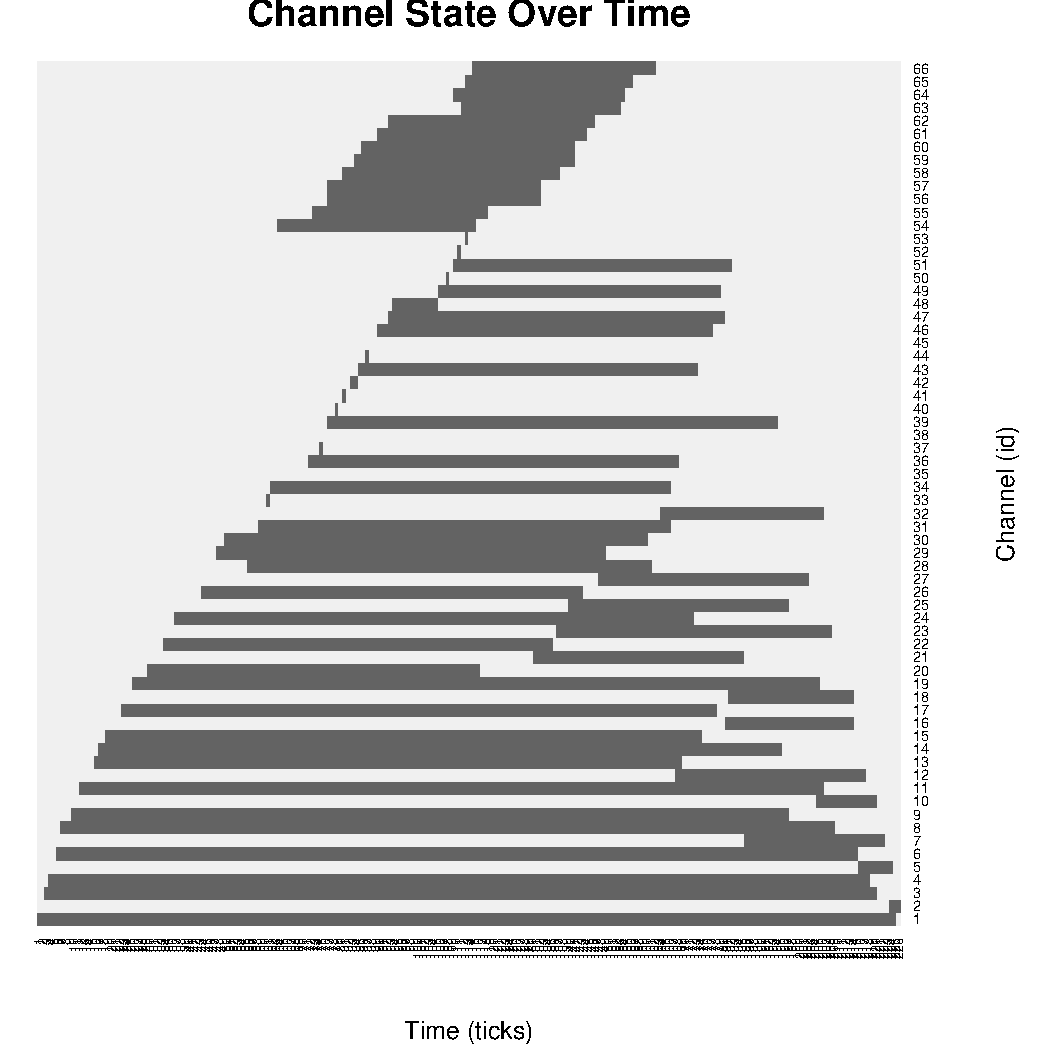
\includegraphics[scale=0.40]{fibonacci-channel-demo.pdf}
    \label{fig:fibonacci-channel-demo-chart}
}%
\subfigure{
    \centering
    \raisebox{20mm}{\footnotesize \BUseVerbatim{FibCode} }
\label{fig:fibonacci-channel-demo-code}
}
    \caption{Parallel Fibonacci implementation and a potential channel graph.}
    \label{fig:fibonacci-channel-demo}
\end{figure}

For example, note the bottom three lines. The first one and the third one are 
all dark until the very end. That first one is the block on the left-hand side
of the Fibonacci merge call, and the third is the response from its subsequent
spawns. The second is never blocked until the end, after we hear back from the
left-hand side. These types of observations will become useful for the later 
scheduler critiques.

\subsection{Scheduler API}\label{sec:results-evaluation-classical}

The ErLam Scheduler API was minimally constructed around the single-step 
scheduling semantics presented earlier in figure~\ref{fig:scheduler-step}.
We were motivated by the simplicity of the description and thus the ability
to bring some formalism to the implementations. That being said, we would still
require the option to observe practical statistics such as runtime overhead 
during our scheduler comparisons. 

\begin{figure}[h!]
    \subfigure[Tick disparity, or the average time between scheduler ticks per 
    LPU, per Task run. Typical ranges tend to spike in groups, which show 
    consistency based on scheduler implementation, rather than OS intervention.]{
        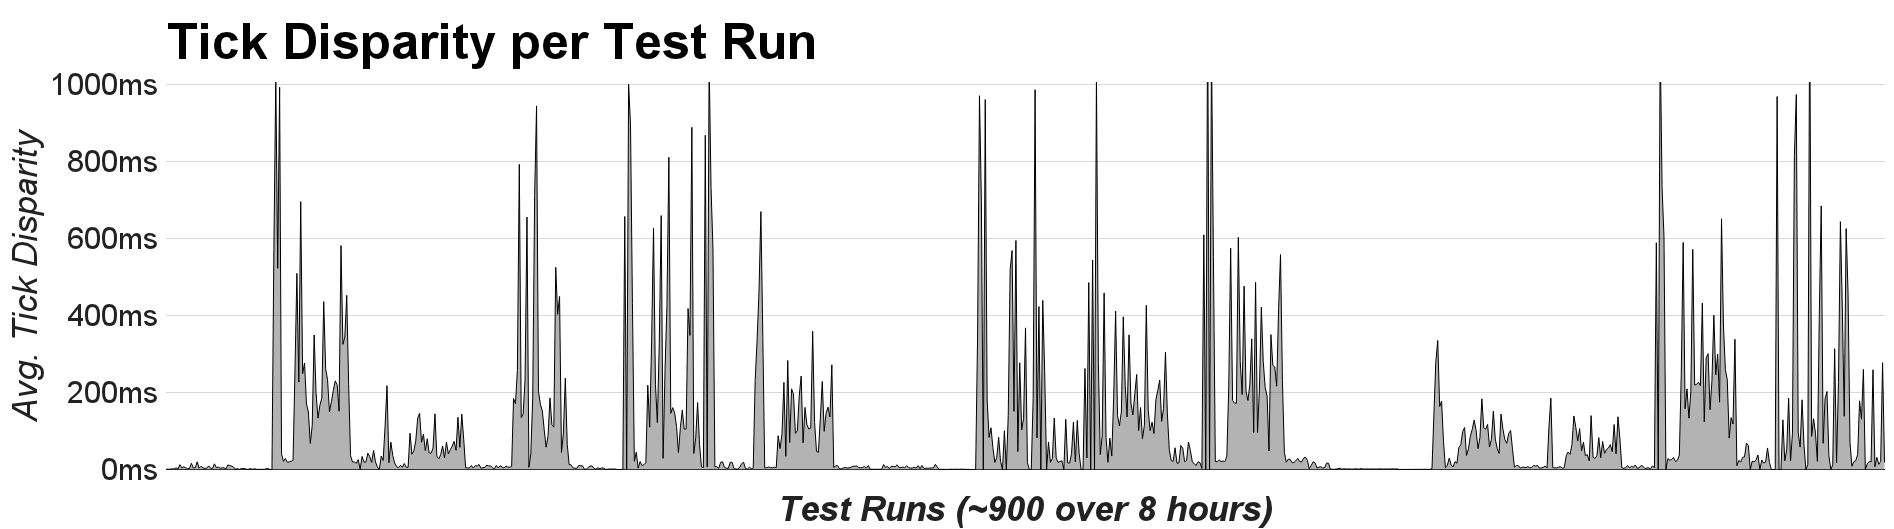
\includegraphics[width=\textwidth]{tick-disparity.png}
        \label{fig:tick-disparity}
    }
    ~
    \subfigure[Tick disparity consistently matches up with increased computation, 
    which is indicitive of inter-scheduler communication requirements.]{
        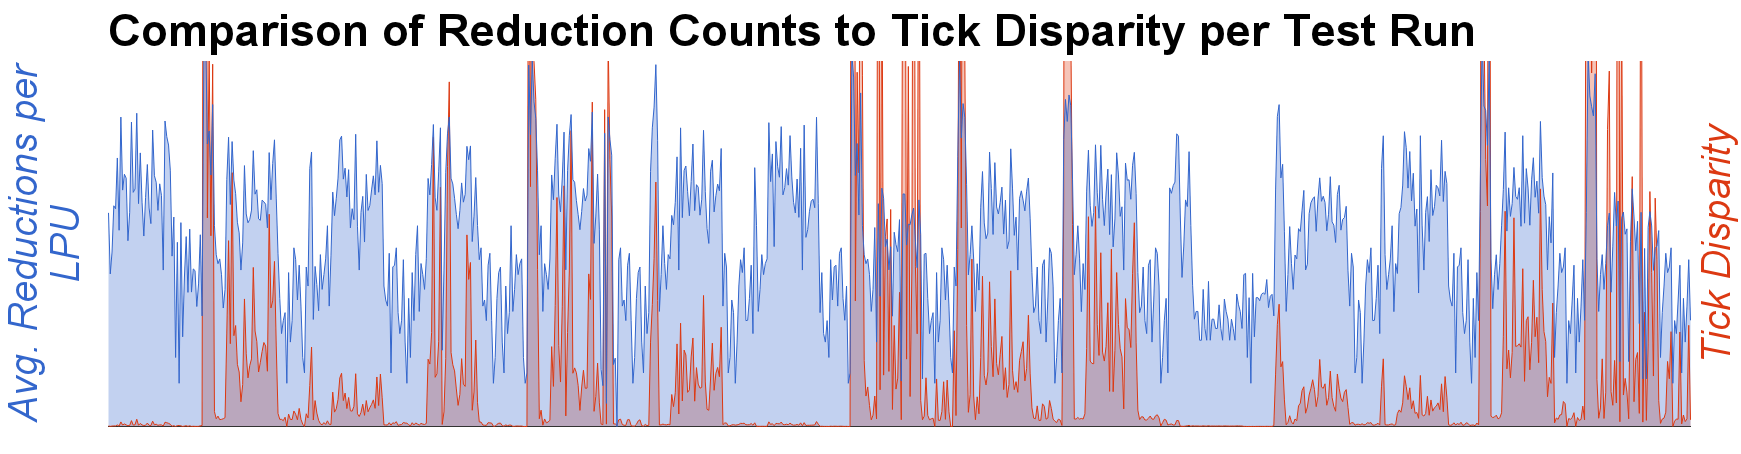
\includegraphics[width=\textwidth]{tick-disparity-to-reductions.png}
        \label{fig:tick-disparity-match}
    }
    \caption{The tick-disparity for over nearly $900$ tests.}
\end{figure}

However,
one of the concerns early on, and as described in section~\ref{sec:runtime log reports}, 
was that the LPUs could greatly differ in the number of ticks they are able to 
provide their process queue. This could be caused by the OS preempting the 
ErLam scheduling thread to execute something else. However, from our tests, we
found these gaps to be minimal and mainly caused by the scheduling implementation
itself. 

Figure~\ref{fig:tick-disparity} shows the average time between ticks averaged over
the LPUs for a large subsection of the tests we ran. We call this average time 
between ticks per LPU the Tick Disparity of the test. From the figure, we notice
obvious clustering, and figure~\ref{fig:tick-disparity-match} leads us to believe this
is primarily caused by spikes in reduction counts. A scheduler chugging on 
processes the entire time, must wait until preemption in-order to handle any 
inter-scheduler communication, as in the case of work-stealing schedulers. Thus,
for our purposes, all talk of tick-disparity could be considered a discussion of
scheduler overhead. As such, comparative analysis of scheduler implementation 
overhead from test case execution would still be a valid comparison with our
design.

Further, to validate that our scheduler implementations functioned as expected 
after translation was another concern. We gave the example of the CML 
Dual-Queue translation ($STDQ$) previously in section~\ref{sec:example the cml scheduler}.
We will now examine its execution and compare it to $STRR$, a single queue naive
scheduler to confirm our understanding.

The key differences we would expect to see in a comparison would be that the CML scheduler
prefers to, and attempts to run the interactive processes first. It would push
all computational processes onto the secondary queue, only promoting them when 
the need arises. To observe this property, we composed the $UserInput_{(T,C)}$ 
test with $ChugMachine_N$ to create an interactivity test primitive 
$Interactivity_{(N,M)}$ (figure~\ref{fig:interactivity-code}). The primitive
launches $ChugMachine_N$ and $M$ instances of $UserInput_{(5,10)}$\footnote{The values
of which were arbitrarily chosen so as to execute for long enough to collect
coherent data.}. We then subsequently ran this primitive with $STRR$ and $STDQ$
using multiple values for $N$ and $M$. Table~\ref{tab:interativity8-16-strr-stdq}
compares an instance of this test set: $Interactivity_{(8,16)}$.

\begin{table}[htp!]
    \centering
    \begin{tabular}{@{}ccc}
        & \multicolumn{2}{c}{$Interactivity_{(8,16)}$} \\ \cline{2-3}
        & \textbf{$STRR$}       & \textbf{$STDQ$}       \\ \cline{2-3} 
\multicolumn{1}{c|}{\rotatebox{90}{\rlap{\textbf{Channel State over Time}}}} & 
    \multicolumn{1}{c|}{\includegraphics[scale=0.32]{tests/interactivity/single/pg_0001.pdf}} & 
    \multicolumn{1}{c|}{\includegraphics[scale=0.32]{tests/interactivity/cml/pg_0001.pdf}} \\ \cline{2-3} 
    \multicolumn{1}{@{}c|}{\rotatebox{90}{\textbf{Communication Density}}}   & 
    \multicolumn{1}{c|}{\includegraphics[scale=0.32]{tests/interactivity/single/pg_0002.pdf}} & 
    \multicolumn{1}{c|}{\includegraphics[scale=0.32]{tests/interactivity/cml/pg_0002.pdf}} \\ \cline{2-3} 
\multicolumn{1}{c|}{\rotatebox{90}{\rlap{\textbf{Reduction Density}}}}       & 
    \multicolumn{1}{c|}{\includegraphics[scale=0.32]{tests/interactivity/single/pg_0003.pdf}} & 
    \multicolumn{1}{c|}{\includegraphics[scale=0.32]{tests/interactivity/cml/pg_0004.pdf}} \\ \cline{2-3} 
\end{tabular}
    \caption{Comparison of $STRR$ and $STDQ$ using Channel State, Reduction and Communication Densities.}
    \label{tab:interativity8-16-strr-stdq}
\end{table}

The Reduction Density graphs explain everything we need to know. The darkened portions
at the beginning of the chart indicate that the $STRR$ scheduler has no regard for the
interactive processes, whereas the $STDQ$ scheduler remains spread out. This seems to be
the opposite if we were to consult the Communication Density charts though. It would appear
here that $STRR$ is getting more frequent communication, and $STDQ$ condenses all 
synchronizations to the end. This is, however, an issue of verbiage, as Interactivity
does not correlate to Communication Density. By this, we mean, $STRR$ is indeed allowing 
communication to happen evenly due to a round-robin schedule, but it is not attending to
spontaneous events (\ie~responses back from $hang$). $STDQ$ on the other-hand pushes all 
inter-process communication backwards as it waits to respond to the $hang$ing processes.

We see this effect more clearly once we compare with the Channel State charts. In $STRR$
we see an even regard for all processes. The tapering of the channel blocks at the 
beginning of the graph is consistent with our understanding of the $merge$-based
successive spawning and the round-robin nature of $STRR$. 
However, $STDQ$ is completely different, and all $UserInput_{(T,C)}$
processes seem to be pushed to the beginning of the execution pool. This is in-fact due
to another difference between the execution styles of the two schedulers: $STDQ$ replaces
the currently running process with the child process it spawned, enqueuing the parent.
We therefore can confirm our understanding, in this case, that the scheduler is reacting
to the test primitives as expected.

The work-stealing mechanics of $MTRRWS$-$SQ$ and $MTRRWS$-$IS$ are another instance for interesting comparison. We've built
two of the cooperativity-conscious schedulers we discuss on top of the $MTRRWS$-$*$ 
process queue implementation. It is this unified queue implementation which allows 
us to toggle between the two implementations. With $MTRRWS$-$SQ$, the process queue
will respond to function calls from schedulers for other LPUs, it will perform a
quick dequeue from the bottom, only blocking the host LPU from accessing the queue
for a minimal amount of time. With $MTRRWS$-$IS$, the process queue goes untouched
by other LPUs, instead the scheduler on the LPU itself will receive the thief messages
and respond during periods between process operations (\eg~during preemption).

To compare these, we would expect to see minor differences in the processes scheduler 
state, but we could expect $MTRRWS$-$IS$ to wait longer for responses from their thief
messages as the victim LPU could be computation-bound. 
But otherwise we would like to make sure the saturation of the cores are 
as identical as possible. In other words, if either method is unable to saturate the 
cores effectually, then it would not be worth further testing (or there is an issue 
with the implementation). 

However, work-stealing schedulers work best if there is a constant probability of 
loosing a process by completion. Our test primitives, as they stand, do not account for
application phases in terms of process quantity or differing longevity. Thus, to effectively examine these
stealing mechanisms, we substitute process loss via completion with process loss via 
channel absorption. Thus, table~\ref{tab:ptree9-10-5-wsis-wssq} gives a comparison of the 
two work-stealing techniques in terms of scheduler state over time and the process 
queue length with a run of $PTree_{(9,10)}$ with the Process Absorption channel turned on.

\begin{table}[htp!]
\centering
    \begin{tabular}{@{}ccc}
        & \multicolumn{2}{c}{$PTree_{(9,10)}$} \\ \cline{2-3}
        & \textbf{$MTRRWS$-$IS$}       & \textbf{$MTRRWS$-$SQ$}       \\ \cline{2-3} 
\multicolumn{1}{c|}{\rotatebox{90}{\rlap{\textbf{Scheduler State}}}} & 
    \multicolumn{1}{c|}{\includegraphics[scale=0.32]{tests/ptree/wsis/pg_0005.pdf}} & 
    \multicolumn{1}{c|}{\includegraphics[scale=0.32]{tests/ptree/wssq/pg_0005.pdf}} \\ \cline{2-3} 
\multicolumn{1}{c|}{\rotatebox{90}{\rlap{\textbf{Process Queue Length}}}}   & 
    \multicolumn{1}{c|}{\includegraphics[scale=0.32]{tests/ptree/wsis/pg_0003.pdf}} & 
    \multicolumn{1}{c|}{\includegraphics[scale=0.32]{tests/ptree/wssq/pg_0003.pdf}} \\ \cline{2-3} 
\end{tabular}
    \caption{Comparison of $MTRRWS$-$IS$ and $MTRRWS$-$SQ$ using Scheduler State and Queue Size.}
    \label{tab:ptree9-10-5-wsis-wssq}
\end{table}

Upon review of this comparison, our initial assumptions have been validated. The process queue
length looks extremely similar. The LPU which owns the initial process maintains the 
largest queue, where all others work steal a single process and work on it. Any gains in
queue size for these LPUs are via channel absorption, but this can not compare with the
initial spawns. We note here that an obvious introduction of smarter work-balancing
would be critical for a realistic or even practically useful scheduler. However, for our
purposes of verifying the work-stealing mechanism and any improvements, this naive implementation is sufficient.

Although the scheduler state comparison, in this instance, does not look consistent with 
the original assumptions. Namely, $MTRRWS$-$IS$ seems not stay in waiting mode as long
as $MTRRWS$-$SQ$ does. However, we can pose two possible reasons for this reaction:
there is an obvious scaling bias introduced by squeezing over $11000$ ticks into the same length
of space as $MTRRWS$-$SQ$ does with $8000$. Additionally, the scheduling reduction quantum for 
this execution was $20$ and all processes were set to chug for only $5$ max, this allows the 
scheduler more opportunity to tend to inter-process communication at a detriment to
the shared-queue implementation due to higher chance of blocked queue access.
The simulation's log was able to support the former rational. It is due to this 
minor increase in speed, that we standardize our tests in this document to 
compare against the $SQ$ stealing mechanism, even if our selected tests showed 
$IS$ as preferred.

\subsection{Channel Implementations}\label{sec:results-channel-implementations}

The above graphs (\eg~table~\ref{tab:interativity8-16-strr-stdq}, and 
table~\ref{tab:ptree9-10-5-wsis-wssq}) were generated, using the CML-like Process 
Absorption channels. We would like to now briefly visualize how a Blocking channel
may operate and effect our visualizations of the application's schedule. In this example 
(table~\ref{tab:interactivity16-8-sq}), we ran the interactivity composure again
to test a large sampling of processes, but some with communication so as to see the 
flow of processes due to absorption.

\begin{table}[htp!]
    \begin{tabular}{@{}ccc}
     \multicolumn{3}{c}{$Interactivity_{(16,8)}$ } \\ \cline{2-3}
        & \textbf{Absorption}       & \textbf{Blocking}       \\ \cline{2-3} 
\multicolumn{1}{c|}{\rotatebox{90}{\rlap{\textbf{Communication Density}}}} & 
    \multicolumn{1}{c|}{\includegraphics[scale=0.32]{tests/interactivity/wssq/ca/pg_0002.pdf}} & 
    \multicolumn{1}{c|}{\includegraphics[scale=0.32]{tests/interactivity/wssq/cb/pg_0002.pdf}} \\ \cline{2-3} 
\multicolumn{1}{c|}{\rotatebox{90}{\rlap{\textbf{Process Queue Length}}}}   & 
    \multicolumn{1}{c|}{\includegraphics[scale=0.32]{tests/interactivity/wssq/ca/pg_0003.pdf}} & 
    \multicolumn{1}{c|}{\includegraphics[scale=0.32]{tests/interactivity/wssq/cb/pg_0003.pdf}} \\ \cline{2-3} 
\end{tabular}
\caption{Comparison of two runs of $Interactivity_{(16,8)}$ on $MTRRWS$-$SQ$ using either Absorption or Blocking swap channels.}
    \label{tab:interactivity16-8-sq}
\end{table}

Note the effects of blocking on the apparent communication density of the 
application. Instead of visualizing only the completion of a swap, this chart
shows any attempted communication, even if it results in a block. Thus if a 
process is allowed to continuously check a required channel for a value, the 
density will increase, as it does for the Blocking channel chart. 

The difference is also apparent in the number of available processes each scheduler has
access to. The lengths of the process queues, fluctuate frequently in both
charts, however the absorption channel does so to quite a large degree. This
is to be expected since any communication which results in a block 
removes a process and any which results in a value returns an extra one.
Whereas the blocking channel chart, the queue size rapidly switches up and
down as it adds its current process and gets the next one. We are also able 
to notice the tell-tail signs of the naive shared-queue work-stealing approach 
in the Blocking channel too (\ie~the single dominate process queue).

We discuss these channel differences further in the next section as we compare 
the cooperativity-conscious schedulers. At this point the operation of the 
blocking scheduler seems unmotivated, however, its effects on the 
Bipartite-Graph Aided Sorting scheduler support the additional study.


\section{Cooperativity Mechanics}\label{sec:results-evaluation-feedback}

We now turn to the discussion of cooperativity-conscious scheduling.
Using our classical scheduler results as a base line we can evaluate 
the presented scheduler mechanics independently. This will give an indication of what
may warrant further investigation, and testing. We direct the readers attention
to appendix~\ref{app:testcases} for full source descriptions of the test 
primitives used throughout this discussion. For any non-explicitly defined
parameter selections, the appendix will have their default values.

However, with the mechanics presented in this section, we wish to highlight particular
distinguishing features of using cooperativity as a metric in a feedback scheduler. 
Namely,
\begin{itemize}
    \item The Longevity-Based Batching scheduler recognizes system interactivity
        and channel communication to batch processes, and longevity detection to
        split them. As such, it is an experiment in using process communication
        behavior to better adapt the system to the level of cooperativity.

    \item The Channel Pinning scheduler is motivation for further examination of
        the work-stealing mechanism. It looks to adapt to the dynamic nature of
        cooperativity by spreading the processes based on common synchronization 
        points.

    \item The Bipartite-Graph Aided Sorting scheduler is motivation to take 
        another look at the channel implementation. Instead of the common 
        absorption channels, a blocking channel allows for scheduler decisions 
        regarding order of process evaluation. This allows for adaptation 
        to possible future cooperative behavior.
\end{itemize}
We therefore restrict the scope of our discussion to the particulars of
each mechanic which directly pertain to cooperativity recognition and
adaptation. We leave it for future work to improve on the trade offs of these
mechanics in practice.

\subsection{Longevity-Based Batching}\label{sec:results-longbatcher}

The Longevity-Based Batcher was an experiment of worst-case scenarios. We
mention in section~\ref{sec:longevity based batching}, that a worst case 
scenario would be one where all processes were seen as long running and 
thus incapable of being batched. Our desire was for it to degrade into 
a common work-stealing mechanism in these scenarios, and this should hold despite 
the channel implementation or time quantum.

We would also like to look at how it would react to a $PRing_N$ execution. This
would be an optimal case as it would batch all processes up to the point where
$N$ is larger than the batch cut-off. Effectively, the longevity batcher would
act like a single threaded scheduler and forgo having to communicate across
processors. Subsequently, we would be able to verify a positive result for this, given
communication and reduction density charts. If a single LPU were completely
saturated while all others were kept in waiting mode, this would indicate the
batching process was a success.

We also would like to look at a number of other possible tests to see the
average cases and how a batching scheduler would handle such applications.
Namely, various $ClusterComm_{(N,M)}$ and $PTree_{(W,N)}$ executions would allow 
for testing of process-absorption based re-batching. We would expect logical
work-groups to form batches, and only show poorer results in instances where
the worker thread computes for longer than the time quantum (as they would be
repeatedly kicked from the batches). Therefore we will instead look at the
effects varying the time-quantum has on the quality of the batching procedure.
We will then look at the process queue lengths and work loads of each LPU.

\subsubsection{Boundary-Case Scenarios}\label{sec:results-longbatcher-worstcase}

We will first consider the worst-case scenario of all computation-bound processes, by 
using $ChugMachine_N$ for several values of $N$ near and 
above $P$, or the max number of LPUs on the machine, which in our case 
is $8$ \footnote{All testing was performed using an Intel Core i7-2820QM.}.  We will 
compare it to the graphs of $MTRRWS$-$SQ$ to determine how close to naive
work-stealing our implementation achieves. We will then subsequently consider
the case of $PRing_N$ for various values of $N$ surrounding the batch size, $B$,
to verify our absorption and batching assumptions.

\begin{table}[h!]
    \centering
    \begin{tabular}{ccccc}
        \multicolumn{5}{c}{$ChugMachine_N$} \\ \cline{2-5}
        & \multicolumn{2}{c}{$MTRRWS$-$SQ$}  & \multicolumn{2}{c}{Long. Batcher}    \\ \cline{2-5}
    \multicolumn{1}{c|}{~} & \multicolumn{1}{c|}{Queue Length} & \multicolumn{1}{c|}{Reduc. Density} & 
        \multicolumn{1}{c|}{Queue Length} & \multicolumn{1}{c|}{Reduc. Density} \\ \cline{2-5}
        \multicolumn{1}{c|}{ \rotatebox{90}{\rlap{$N=P=8$}~} } & 
    \multicolumn{1}{c}{\includegraphics[scale=0.15]{tests/chugmachine/wssq/8/pg_0003.pdf}} &
        \multicolumn{1}{c|}{\includegraphics[scale=0.15]{tests/chugmachine/wssq/8/pg_0004.pdf}} & 
    \multicolumn{1}{c}{\includegraphics[scale=0.15]{tests/chugmachine/longbatcher/8/pg_0003.pdf}}&
        \multicolumn{1}{c|}{\includegraphics[scale=0.15]{tests/chugmachine/longbatcher/8/pg_0004.pdf}} \\ \cline{2-5}

        \multicolumn{1}{c|}{ \rotatebox{90}{\rlap{$N=2P=16$}~} } & 
    \multicolumn{1}{c}{\includegraphics[scale=0.15]{tests/chugmachine/wssq/16/pg_0003.pdf}} &
        \multicolumn{1}{c|}{\includegraphics[scale=0.15]{tests/chugmachine/wssq/16/pg_0004.pdf}} & 
    \multicolumn{1}{c}{\includegraphics[scale=0.15]{tests/chugmachine/longbatcher/16/pg_0003.pdf}}&
        \multicolumn{1}{c|}{\includegraphics[scale=0.15]{tests/chugmachine/longbatcher/16/pg_0004.pdf}} \\ \cline{2-5}
 
        \multicolumn{1}{c|}{ \rotatebox{90}{\rlap{$N=4P=32$}~} } & 
    \multicolumn{1}{c}{\includegraphics[scale=0.15]{tests/chugmachine/wssq/32/pg_0003.pdf}} &
        \multicolumn{1}{c|}{\includegraphics[scale=0.15]{tests/chugmachine/wssq/32/pg_0004.pdf}} & 
    \multicolumn{1}{c}{\includegraphics[scale=0.15]{tests/chugmachine/longbatcher/32/pg_0003.pdf}}&
        \multicolumn{1}{c|}{\includegraphics[scale=0.15]{tests/chugmachine/longbatcher/32/pg_0004.pdf}} \\ \cline{2-5}
 
\end{tabular}
\caption{Comparison of $ChugMachine_N$ spread on the Longevity-Batching Scheduler and $MTRRWS$-$SQ$.}
    \label{tab:chugmachine-longbatcher-testing}
\end{table}

First, table~\ref{tab:chugmachine-longbatcher-testing} visualizes a
$ChugMachine_N$ comparison with the Longevity-Based Batcher and $MTRRWS$-$SQ$. 
With the Longevity-Batcher, we can observe the common work-stealing behavior 
with a primary LPU and minimal queue lengths on all others. It initially spreads
work out as the primary queue continues to chug. However, the $MTRRWS$-$SQ$ seem
to have an easier time of stealing the primary process which is in the process of
spawning the worker threads. Therefore the spread seems to be consistently more
even.

We hypothesized that the mechanism we were using for spawning into a batch was 
somehow making it improbable that it would be migrated to another core. In fact 
there are two mechanisms we have implemented for Long. Batcher to handle a spawn.
\begin{itemize}
    \item In `singleton' batching mode, if a spawn would cause the current batch 
    to be $\geq B$ then a new batch is created for the child and set as the 
    current batch. The old batch with the parent is placed on the queue.

    \item In `push-back' batching mode, if a spawn forces a new batch to be made, 
    we push the current batch onto the queue and keep the current process in the 
    same batch as the new child. This will keep the parent close to its 
    immediate child and also allow it to be quickly re-tested for more new spawns.
\end{itemize}
Note that in `push-back' mode, the scheduler with the primary process will never
be in a position to give it up until all children are finished being spawned. This
was our default for the Longevity Batcher in the above test. As such, 
table~\ref{tab:chugmachine-longbatcher-singleton-testing} shows a re-execution of 
$PRing_{32}$ with `singleton'-mode turned on.

\begin{table}[ht!]
    \centering
    \begin{tabular}{ccc}
        & \multicolumn{2}{c}{$ChugMachine_N$} \\ \cline{2-3}
        \multicolumn{1}{c|}{~} & \multicolumn{1}{c|}{Queue Length} & \multicolumn{1}{c|}{Reduc. Density} \\ \cline{2-3}
\multicolumn{1}{c|}{\rotatebox{90}{\rlap{$N=P=8$}~} } & 
    \multicolumn{1}{c}{\includegraphics[scale=0.20]{tests/chugmachine/longbatcher/32_singleton/pg_0003.pdf}}&
    \multicolumn{1}{c|}{\includegraphics[scale=0.20]{tests/chugmachine/longbatcher/32_singleton/pg_0004.pdf}} \\ \cline{2-3}
\end{tabular}
\caption{Re-run of $ChugMachine_N$ with Longevity-Batching Scheduler in `singleton' batching mode.}
    \label{tab:chugmachine-longbatcher-singleton-testing}
\end{table}

Despite giving it every opportunity to increase the spread, the parent
process is a short-running process (as it would spawn a new process before it would
hit its time quantum). Therefore, while it does have a higher chance to get stolen,
it will also have a higher chance of staying batched until it reaches the point where it hangs
for completion. This obviously limits our chances at immediate parallelism. The 
conclusion that Longevity-Based Batching is $MTRRWS$-$SQ$ in the worst-case scenario 
is therefore not quite true.

However, that being said, the spawning mechanism differences do point to 
some interesting application behaviors. Namely, while the `singleton'-mode was advantageous 
for this application start up, it may not be for all. For example, a program which
rapidly spawns micro processes to get multiple small tasks done, may find the
`push-back' batching mode to be preferred.

\begin{table}[htp!]
    \centering
    \begin{tabular}{@{}cccc}
        & \multicolumn{3}{c}{$PRing_N$} \\ \cline{2-4}
    & $N=P=8$ & $N=B=10$ & $N=2*B=20$     \\ \cline{2-4} 
        \multicolumn{1}{c|}{\rotatebox{90}{\rlap{\textbf{Reduction Density}}}} & 
    \multicolumn{1}{c|}{\includegraphics[scale=0.20]{tests/pring/longbatcher/8/pg_0004.pdf}} & 
    \multicolumn{1}{c|}{\includegraphics[scale=0.20]{tests/pring/longbatcher/10/pg_0004.pdf}} & 
    \multicolumn{1}{c|}{\includegraphics[scale=0.20]{tests/pring/longbatcher/20/pg_0004.pdf}} \\ \cline{2-4} 
\end{tabular}
\caption{Comparison of different sized $PRing_N$ on a the Longevity Batching Scheduler with batch size $B=10$.}
    \label{tab:pring-longbatcher-testing}
\end{table}

Finally, table~\ref{tab:pring-longbatcher-testing} visualizes the reduction 
densities of several $PRing_N$ executions using the Longevity-Based Batcher 
with Absorption Channels turned on. We note the obvious agreement with our 
assumption as the entire $PRing_N$ gets absorbed into a single batch and 
contained to a single core.  The spill-over at the beginning of the $PRing_{20}$
execution was due to the spawning of more than $B$ processes. However, after
their absorption via communication, the Longevity-Based Batcher was free to
maintain all processes in the same batch without harming parallelism.

While the scheduler does not reduce exactly to $MTRRWS$-$*$ as hypothesized, this result 
shows an improvement over alternative batching approaches as we explicitly relax the 
constraints of system-wide batching. Any lack of parallelism is caught by the check 
for longevity.

\subsubsection{Time-Quantum Effects}\label{sec:results-longbatcher-timequantum}

Of the average scenarios we are interested in only the effects of our time quantum
on the quality and level of batching in each scenario; as batching has been examined 
before in terms of alternative metrics. We will look at the same test case, 
$PTree_{(4,8)}$ as the number of work-groups ($4$) is less than the number of LPUs 
and the number of processes per work-group ($8$) is lower than the batch-size limits 
($10$). 

The rational for this seemingly arbitrary test-case selection is two fold. First,
the supervisory processes are all short-running and may force the logical batches 
to be inflated in size by at least two (\ie~thus the reduction in processes in 
work-groups). Then secondly, when we reduce the time quantums to well below the
worker-thread's execution spawn (before it hits a sync), the number of batches
will increase substantially and we would like to see the scheduling effects. Having
a 2-to-1 number of LPUs to potential batches seemed logical.

\begin{table}[htp!]
    \centering
    \begin{tabular}{ccccc} & \multicolumn{4}{c}{ $PTree_{(4,8)}$ } \\ \cline{2-5}
    \multicolumn{1}{c}{\textbf{Time}} & \multicolumn{2}{c}{ $MTRRWS$-$SQ$ } & \multicolumn{2}{c}{ Long. Batcher} \\ \cline{2-5}
    \multicolumn{1}{c|}{\textbf{Quantum}} & \textbf{Chan. State} & \multicolumn{1}{c|}{\textbf{Reduc. Density}} 
                                                & \textbf{Chan. State} & \multicolumn{1}{c|}{\textbf{Reduc. Density}} \\ \cline{1-5}
    \multicolumn{1}{c|}{$R=30$} &  \multicolumn{1}{c}{\includegraphics[scale=0.15]{tests/ptree/wssq/ca30r/pg_0003.pdf}} &
                                   \multicolumn{1}{c|}{\includegraphics[scale=0.15]{tests/ptree/wssq/ca30r/pg_0004.pdf}} &
                                   \multicolumn{1}{c}{\includegraphics[scale=0.15]{tests/ptree/lbb/ca30r/pg_0003.pdf}} &
                                   \multicolumn{1}{c|}{\includegraphics[scale=0.15]{tests/ptree/lbb/ca30r/pg_0004.pdf}} \\ \cline{1-5}

    \multicolumn{1}{c|}{$R=40$} &  \multicolumn{1}{c}{\includegraphics[scale=0.15]{tests/ptree/wssq/ca40r/pg_0003.pdf}} &
                                   \multicolumn{1}{c|}{\includegraphics[scale=0.15]{tests/ptree/wssq/ca40r/pg_0004.pdf}} &
                                   \multicolumn{1}{c}{\includegraphics[scale=0.15]{tests/ptree/lbb/ca40r/pg_0003.pdf}} &
                                   \multicolumn{1}{c|}{\includegraphics[scale=0.15]{tests/ptree/lbb/ca40r/pg_0004.pdf}} \\ \cline{1-5}

    \multicolumn{1}{c|}{$R=50$} &  \multicolumn{1}{c}{\includegraphics[scale=0.15]{tests/ptree/wssq/ca50r/pg_0003.pdf}} &
                                   \multicolumn{1}{c|}{\includegraphics[scale=0.15]{tests/ptree/wssq/ca50r/pg_0004.pdf}} &
                                   \multicolumn{1}{c}{\includegraphics[scale=0.15]{tests/ptree/lbb/ca50r/pg_0003.pdf}} &
                                   \multicolumn{1}{c|}{\includegraphics[scale=0.15]{tests/ptree/lbb/ca50r/pg_0004.pdf}} \\ \cline{1-5}
    \end{tabular}
    \caption{Comparison of $PTree_{(4,8)}$ running with the Longevity-Based 
        Batching Scheduler and $MTRRWS$-$SQ$ at different time-quantums.} 
    \label{tab:ptree-longbatcher-testing}
\end{table}

Table~\ref{tab:ptree-longbatcher-testing} notes the gradual shift of the number of 
logical batches formed in the Longevity-Based Batcher. For the lower values of 
$R$, the max reduction count per round, the number of batches rose substantially and
began to look like $MTRRWS$-$SQ$. For all subsequent quantum selections there was
a stead drop in the the sizes of the LPUs' process queues, until at $R=50$ we 
see that no queue goes above size $1$, indicating each work-group has been clustered.

We close on the note that the selection of the time-quantum can easily be set 
heuristically, modified between rounds, and possibly on a per-LPU basis. It would
need to take into account the average distance between synchronization points
of the processes in its batch queue. Using that, it would be able to determine if
a particular process posed a greater than average threat to the parallelism of the 
system, and subsequently push it into a singleton batch.

\subsection{Channel Pinning}\label{sec:results-channelpinner}

This cooperativity-conscious scheduler attempts to group processes based on the 
channels they communicate frequently with. It does so by pinning the channels to
the set of LPUs based on a particular spreading algorithm, and then piggy backs
on the channel implementation to relocate the processes using absorption. This 
has the potential effect of compensating for frequent, and especially uniform,
communicating processes ahead of time.

As mentioned in section~\ref{sec:channel pinning}, our primary interest in this 
scheduler is the selective stealing technique used along with its ability to 
maintain LPU saturation with channel pinning and process absorption. Its design 
is based on recognizing cooperativity where it exists. If two processes communicate
with different channels, their likelihood of being reliant on one another decreases.
As such, we will look at the two extremes for communication behavior, completely random 
and then completely uniform. That is, a system which has no predicable or
repeatable behavior, and then a system were the past will directly inform the future. 

We therefore utilize $ClusterComm_{(N,M)}$ for its random behavior, and turn to the 
$Interactivity_{(N,0)}$ composure to simulate uniform communication. In other words,
we will have $N$ uniform communicating units which compute and are stolen separately 
($UserInput_{(T,C)}$). As such, we hope to highlight the scheduler's ability to 
consistently saturate the cores with work under both the best (uniform) and worst
case (random) conditions. We leave it to future research for a discussion of the 
possible channel spreading techniques and work-stealing mechanisms, along with their
effects in practical feedback schedulers.


\subsubsection{Random and Uniform Communication}\label{sec:results-cp-rand-uniform}

We begin our communication behavior tests by observing the queue lengths and reduction
densities during the execution of a particular pair of tests: 
$Interactivity_{(20,0)}$ and $ClusterComm_{(20,5)}$.\footnote{
            We chose these tests due to being in the upper-bound of process quantity of
            the tests we ran. They would be the best bet to demonstrate saturation.}
We subsequently compare results of the Channel Pinning scheduler with those of 
$MTRRWS$-$SQ$ via table~\ref{tab:cp-compare-rand-uniform-ca}. 

\begin{table}[htp!]
    \centering
\begin{tabular}{@{}ccccc}
    & \multicolumn{2}{c|}{$Interactivity_{(20,0)}$} & \multicolumn{2}{c}{$ClusterComm_{(20,5)}$} \\ \cline{2-5} 
 & \multicolumn{1}{c}{$MTRRWS$-$SQ$}       & \multicolumn{1}{c|}{Channel Pinning} 
 & \multicolumn{1}{c}{$MTRRWS$-$SQ$}       & \multicolumn{1}{c}{Channel Pinning} \\ \cline{2-5} 
 
\multicolumn{1}{c|}{\rotatebox{90}{\rlap{~~Comm. Density}}} &
    \multicolumn{1}{c}{\includegraphics[scale=0.15]{tests/interactivity/20/wssq/ca/pg_0002.pdf}} & 
    \multicolumn{1}{c|}{\includegraphics[scale=0.15]{tests/interactivity/20/cp/ca/pg_0002.pdf}} &
    \multicolumn{1}{c}{\includegraphics[scale=0.15]{tests/clustercomm/20/wssq/ca/pg_0002.pdf}} &
    \multicolumn{1}{c|}{\includegraphics[scale=0.15]{tests/clustercomm/20/cp/ca/pg_0002.pdf}} \\

 
\multicolumn{1}{c|}{\rotatebox{90}{\rlap{~~Queue Length}}} &
    \multicolumn{1}{c}{\includegraphics[scale=0.15]{tests/interactivity/20/wssq/ca/pg_0003.pdf}} & 
    \multicolumn{1}{c|}{\includegraphics[scale=0.15]{tests/interactivity/20/cp/ca/pg_0003.pdf}} &
    \multicolumn{1}{c}{\includegraphics[scale=0.15]{tests/clustercomm/20/wssq/ca/pg_0003.pdf}} &
    \multicolumn{1}{c|}{\includegraphics[scale=0.15]{tests/clustercomm/20/cp/ca/pg_0003.pdf}} \\

\multicolumn{1}{c|}{\rotatebox{90}{\rlap{Reduc. Density}}} &
    \multicolumn{1}{c}{\includegraphics[scale=0.15]{tests/interactivity/20/wssq/ca/pg_0004.pdf}} & 
    \multicolumn{1}{c|}{\includegraphics[scale=0.15]{tests/interactivity/20/cp/ca/pg_0004.pdf}} &
    \multicolumn{1}{c}{\includegraphics[scale=0.15]{tests/clustercomm/20/wssq/ca/pg_0004.pdf}} &
    \multicolumn{1}{c|}{\includegraphics[scale=0.15]{tests/clustercomm/20/cp/ca/pg_0004.pdf}} \\ \cline{2-5}

\end{tabular}
\caption{Comparison of Random and Uniform synchronization for $MTRRWS$-$SQ$ and 
the Channel Pinning Scheduler on Absorption Channels.}
\label{tab:cp-compare-rand-uniform-ca}
\end{table}

We will start our discussion with the executions of $Interactivity_{(20,0)}$.
Starting at the bottom and working up, we notice the level of saturation the 
channel pinning scheduler achieves over $MTRRWS$-$SQ$. Its slightly denser,
despite the same general execution time (in tick quantity). However, the channel
pinning scheduler still maintains the tell-tail signs of the underlying 
naive work-stealing approach via the single primary LPU. The queue lengths'
confirm this with much more activity on all secondary LPUs. Despite the 
unevenness, we see a much uniform attention to the state of channels.
Communication Densities show an obvious front-loading effect when there is 
predictable communication happening. 

However, for $ClusterComm_{(20,5)}$ we see no marked difference in the channel
pinning scheduler's spread. In fact it looks to take longer to saturate the 
cores than a normal work-stealer. Possibly due to the work-stealing by channel-id
not matching a process until much later. Despite this, it looks as though there 
was very little detriment, as the applications completed in roughly similar time.

Note for these tests we used the $even$ spreading algorithm 
(section~\ref{sec:channel pinning}) to calculate our next LPU for pinning instead of
$same$. Our $ClusterComm_{(N,M)}$ test primitive creates all channels in the same
process before spawning all workers, so pinning all channels to the primary LPU 
would have been a detriment. Thus to give the tests the best possible chance
at succeeding, we chose our most efficient spreading algorithm.

\subsection{Bipartite-Graph Aided Sorting}\label{sec:results-smartsort}

The Bipartite-Graph Aided Sorting Scheduler attempts to observe the effects
process queue order has on the scheduling of an application. It utilizes a mapping
of the process set to the channel set and sorts its process queue based on 
the known edges between the sets. With this scheduler, our primary focus was
in the recognition of cases which lend themselves to sorting, as such we 
leave a critique of sorting algorithms and sorting frequencies to future work
in this field.

We utilize the same tests as performed in the previous section, to visualize the
scheduling differences of random and uniform communication behaviors. 
Although, the Sorting scheduler was the most complicated of the cooperativity 
conscious schedulers to test and evaluate. In fact, we needed to stray from our 
test primitives and examine one of our original example applications, the 
Parallel Fibonacci, to properly test it. This is due to none of our tests
being dominantly dependent on process order (\ie~the majority of processes in the
test primitives are worker threads and only $1$ process is waiting on them to
complete), thus Parallel Fibonacci was poised to be a best-case scenario.

\subsubsection{Random and Uniform Communication}\label{sec:results-smartsort-rand-uniform}

We ran $Interactivity_{(20,0)}$ and $ClusterComm_{(20,5)}$ like before, using Absorption
channels first. We hypothesized that this channel implementation would provide
little improvement and the overhead involved with sorting the process queue would
be wasted as soon as a channel was absorbed and effectively reordered. 
Table~\ref{tab:ss-compare-rand-uniform-ca} presents these executions, and they
meet expectation.

\begin{table}[tp!]
    \centering
    \begin{tabular}{@{}ccc}
        & $MTRRWS$-$SQ$       & Sorting Scheduler       \\ \cline{2-3} 
\multicolumn{1}{c|}{\rotatebox{90}{\rlap{~~~~~~~~~~~~$Interactivity_{(20,0)}$}}} & 
    \multicolumn{1}{c|}{\includegraphics[scale=0.32]{tests/interactivity/20/wssq/ca/pg_0001.pdf}} & 
    \multicolumn{1}{c|}{\includegraphics[scale=0.32]{tests/interactivity/20/ss/ca/pg_0001.pdf}} \\ \cline{2-3} 
\multicolumn{1}{c|}{\rotatebox{90}{\rlap{~~~~~~~~~~~~$ClusterComm_{(20,5)}$}}}   & 
    \multicolumn{1}{c|}{\includegraphics[scale=0.32]{tests/clustercomm/20/wssq/ca/pg_0001.pdf}} & 
    \multicolumn{1}{c|}{\includegraphics[scale=0.32]{tests/clustercomm/20/ss/ca/pg_0001.pdf}} \\ \cline{2-3} 
\end{tabular}
\caption{Comparison of Random and Uniform synchronization for $MTRRWS$-$SQ$ and 
the Bipartite-Graph Aided Sorting Scheduler using Absorption Channels.}
    \label{tab:ss-compare-rand-uniform-ca}
\end{table}

Note very little difference in the charts on either side of the median.
Absorption channels remove any chance the scheduler may have of improving the 
runtime quality of the application. Blocking channels, on the other hand, can leak
hints to the scheduler, which it may then use to predict the future.
Table~\ref{tab:ss-compare-rand-uniform-cb} displays a re-execution of the 
above tests utilizing Blocking channels instead.

\begin{table}[tp!]
    \centering
    \begin{tabular}{@{}ccc}
        & $MTRRWS$-$SQ$       & Sorting Scheduler       \\ \cline{2-3} 
\multicolumn{1}{c|}{\rotatebox{90}{\rlap{~~~~~~~~~~~~$Interactivity_{(20,0)}$}}} & 
    \multicolumn{1}{c|}{\includegraphics[scale=0.32]{tests/interactivity/20/wssq/cb/pg_0001.pdf}} & 
    \multicolumn{1}{c|}{\includegraphics[scale=0.32]{tests/interactivity/20/ss/cb/pg_0001.pdf}} \\ \cline{2-3} 
\multicolumn{1}{c|}{\rotatebox{90}{\rlap{~~~~~~~~~~~~$ClusterComm_{(20,5)}$}}}   & 
    \multicolumn{1}{c|}{\includegraphics[scale=0.32]{tests/clustercomm/20/wssq/cb/pg_0001.pdf}} & 
    \multicolumn{1}{c|}{\includegraphics[scale=0.32]{tests/clustercomm/20/ss/cb/pg_0001.pdf}} \\ \cline{2-3} 
\end{tabular}
\caption{Comparison of Random and Uniform synchronization for $MTRRWS$-$SQ$ and 
the Bipartite-Graph Aided Sorting Scheduler on Blocking Channels.}
    \label{tab:ss-compare-rand-uniform-cb}
\end{table}

While these charts seem fairly similar there are two things of note. Random
communication does not lead to much improvement, despite the apparent
difference in execution time. Whereas, if there is a uniform set of processes 
which communicate frequently, the sorting algorithm can place them next to
one another in the process queue to quickly unblock the channel. This result 
is consistent with our hypothesis. However, it is much more apparent in the
following section.

\subsubsection{Optimal-Case Scenario}\label{sec:results-smartsort-optimal}

We now compare the execution of the Parallel Fibonacci application with the
Sorting scheduler and $MTRRWS$-$SQ$. To do so, we look at the Channel State
graphs to examine the lengths of time channels are blocked. A positive result
would be one where the Sorting scheduler visually reduces the length of 
time channels are blocked on average. Table~\ref{tab:ss-compare-fib} presents
this comparison. We attempted to find the $10^{th}$ Fibonacci number, using 
the algorithm presented in figure~\ref{fig:fibonacci-channel-demo} using the
default sort frequency and algorithm.

\begin{table}[tp!]
    \centering
    \begin{tabular}{@{}ccc}
    & $MTRRWS$-$SQ$ & Sorting Scheduler  \\ \cline{2-3} 
        \multicolumn{1}{c|}{\rotatebox{90}{\rlap{\textbf{Reduction Density}}}} & 
    \multicolumn{1}{c|}{\includegraphics[scale=0.30]{tests/pfib/wssq/pg_0001.pdf}} & 
    \multicolumn{1}{c|}{\includegraphics[scale=0.30]{tests/pfib/ss/pg_0001.pdf}} \\ \cline{2-3}
\end{tabular}
\caption{Channel State comparison of Parallel Fibonacci executed on $MTRRWS$-$SQ$ 
    and the Bipartite-Graph Aided Sorting Scheduler. }
    \label{tab:ss-compare-fib}
\end{table}

We mention now, as we did in section~\ref{sec:results-evaluation-classical},
the effects of scaling in the graph. The number of ticks visualized in the 
Sorting scheduler's graph is exactly $51$, whereas in the other it is over
$1000$. The fact that they look identical at this scale is a testament to the
fact that the reordering of process queues is an effective means by which to
speed up execution. Ultimately this prompts further discussion on the channel
implementation.

\section{A Comment on Swap Channels}\label{sec:results-swap-channels}

Swap channels provided a number of benefits on the side of the language 
designer. They reduce the complexity of channel implementation, and as shown, 
they lend themselves to a number of possible designs. We demonstrated just two 
possible implementations, the Blocking and Absorption channels. As such, the 
concept of a swap channel as a language primitive is extremely attractive. 
However, swapping poses some problems for realistic applications which we would
now like to discuss.

\begin{figure}[tp!]
\centering
\inputminted[frame=lines,fontsize=\footnotesize]{csharp}{code/badclustercomm.els}
\caption{A naive but ineffectual $ClusterComm_{(N,M)}$ implementation.} 
\label{fig:bad-clustercomm}
\end{figure}

First, a swap channel does not lend itself to a level of fairness that would be
expected by a programmer. We lead with our implementation of 
$ClusterComm_{(N,M)}$ as example, which due to being on top of swap channels, 
was made to be much more enigmatic. Figure~\ref{fig:bad-clustercomm} gives an
example implementation of $ClusterComm_{(N,M)}$. Note the third parameter to
the application, which denotes the number of time's each of the $N$ processes
should communicate. The system therefore blocks until all processes synchronize
$X$ times before quiting.

Due to this, we must pose several restrictions on the possible values of $N$ and
$M$. Namely, $N$ must be an even number, since all processes would need to have a 
partner to swap with, and $M$ must be no greater than $\lfloor N/2 \rfloor$, any
more and it would be possible for a process to hang indefinitely.

However, these two restrictions are not enough to guarantee the process terminates.
In fact, most runs of this application, with any value of $N > 2$ would most 
likely hang forever. This is due to the bias our program creates when spawning
processes, as well as the type of fairness the swap channel semantics provides.

First, our bias we introduce is merely because we cannot batch spawn a set of
processes at the same time. As such we will spawn one process at a time which
may get a chance to run before all others. As such the first several processes
may reach their synchronization limit before we are even done spawning the rest
of the processes. Due to this, we may have a case where all but $M$ processes
have completed, and thus all channels are blocked indefinitely.

Secondly, the channel semantics have no inherent preference for unseen 
or new processes. The scheduler may easily get in a loop of running the same
subset of processes repeatedly, this would have the same effect as the above
even if we were able to solve the bias problem. As such, this is inherently an
issue with the capabilities of swap channels. 

Thus, the best we can do for $ClusterComm_{(N,M)}$, is to run until at least 
$N-M$ processes have met their quota. Note this approach is only acceptable 
under Symmetric message passing constructs. In asymmetrical, even if there was
a guarantee of an equal number of senders and receivers, all senders could be
blocked on one channel while all receivers could be blocked on another. 

But this issue points to another problem with swap channels, insofar as they do
not lend themselves to being primitives at all. Due to this fairness issue, a 
language with swap channels would be unable to build the asymmetrical constructs
most user's would like. As such, they have been useful merely for simulation 
purposes.

However, for further simulation of cooperativity, it may be advantageous to also 
consider the directionality of communication. The recognition of consumer and 
producer processes may lend itself to further gains as the recognition of 
communication and computation bound processes did. This is not to say all gains
in utilizing pure synchronization have been obtained. 
